%! suppress = MissingImport
%! suppress = MissingLabel
%! suppress = LineBreak

% CLI args https://tex.stackexchange.com/a/1501
\newif\ifhandout
\input{flags}

%! suppress = MissingLabel
%! suppress = DocumentclassNotInRoot
%! suppress = DiscouragedUseOfDef

% * Make friends tikz & colors
%   https://en.wikibooks.org/wiki/LaTeX/Colors
% * To enable vertical top alignment globally
%   https://tex.stackexchange.com/questions/9889/positioning-content-at-the-top-of-a-beamer-slide-by-default
% * Set handout from CLI
%   https://tex.stackexchange.com/a/1501
\ifhandout
\documentclass[usenames, dvipsnames, handout]{beamer} % https://tex.stackexchange.com/questions/224091/beamer-how-to-disable-pause-temporarily
\else
\documentclass[usenames, dvipsnames]{beamer}
\fi
% ------------------------------------------------

% Graphics
\usepackage{color}
\usepackage{tabularx}
\usepackage{tikz}
% https://tikz.dev/tikz-graphs
\usetikzlibrary{positioning, shapes.geometric, arrows, automata, graphs}
\tikzset{
    expr/.style={ellipse, draw=gray!60, fill=gray!5, very thick, minimum size=7mm, yshift=0.7cm},
    hexpr/.style={ellipse, draw=gray!60, fill=blue!15, very thick, minimum size=7mm, yshift=0.7cm},
    stmt/.style={rectangle, draw=gray!60, fill=gray!5, very thick, minimum size=5mm, yshift=0.7cm},
    decl/.style={rectangle, draw=blue!60, fill=gray!5, very thick, minimum size=5mm, yshift=0.7cm},
    hdecl/.style={rectangle, draw=blue!60, fill=blue!15, very thick, minimum size=5mm, yshift=0.7cm},
    subtree/.style={shape border rotate=90, isosceles triangle, draw=gray!60, fill=gray!5, very thick, minimum size=5mm, yshift=0.0cm},
}
\usepackage{blkarray}
\usepackage{graphicx}
\usepackage{forest} % https://tex.stackexchange.com/questions/198405/how-to-change-the-color-of-subtrees-in-tikz-qtree
% ------------------------------------------------

% Math
\usepackage{amsmath, amsfonts}
\usepackage{amssymb}
\usepackage{proof}
\usepackage{mathrsfs}
% Crossed-out symbols
% https://tex.stackexchange.com/questions/75525/how-to-write-crossed-out-math-in-latex
\usepackage[makeroom]{cancel}
\usepackage{mathtools}
% ------------------------------------------------

% Additional font sizes
% https://www.overleaf.com/learn/latex/Questions/How_do_I_adjust_the_font_size%3F
\usepackage{moresize}
% Additional colors
% https://www.overleaf.com/learn/latex/Using_colours_in_LaTeX
\usepackage{xcolor}
% Textual math symbols
\usepackage{textcomp}
% ------------------------------------------------

% Language
\usepackage[utf8] {inputenc}
\usepackage[T2A] {fontenc}
\usepackage[english, russian] {babel}
\usepackage{indentfirst, verbatim}
\usetikzlibrary{cd, babel}
% ------------------------------------------------

% Fonts: https://sites.math.washington.edu/~reu/docs/latex_symbols.pdf
\usepackage{stmaryrd}
\usepackage{cmbright}
\usepackage{wasysym}
\usepackage[weather]{ifsym} % https://tex.stackexchange.com/questions/100424/how-to-use-the-ifsym-package
% https://tex.stackexchange.com/questions/615300/pdflatex-builtin-glyph-names-is-empty
\pdfmapline{=dictsym DictSym <dictsym.pfb}
\pdfmapline{=pigpen <pigpen.pfa}
\usepackage{dictsym}
% ------------------------------------------------

% Code
% * Needs -shell-escape build flag
%   https://tex.stackexchange.com/questions/99475/how-to-invoke-latex-with-the-shell-escape-flag-in-texstudio-former-texmakerx
% * Set build directory
%   https://tex.stackexchange.com/questions/339931/latex-minted-package-using-custom-output-directory-build
\usepackage{minted}
\setminted{xleftmargin=\parindent, autogobble, escapeinside=\#\#}
% ------------------------------------------------

% Template
\usetheme{CambridgeUS}
\usecolortheme{dolphin}
% https://tex.stackexchange.com/questions/231439/beamer-how-to-make-font-larger-for-page-numbers
\setbeamerfont{headline}{size=\scriptsize}
\setbeamerfont{footline}{size=\scriptsize}
% Remove heddline
% https://tex.stackexchange.com/questions/33146/how-could-i-remove-a-header-in-a-beamer-presentation
%\setbeamertemplate{headline}{}
% Slide sizes
% https://tex.stackexchange.com/questions/56768/how-to-set-a-small-default-font-size-with-beamer
%\geometry{paperwidth=140mm,paperheight=105mm} % 4:3
\geometry{paperwidth=168mm,paperheight=105mm} % 16:10
% Remove navigation bar
% https://stackoverflow.com/questions/3210205/how-to-get-rid-of-navigation-bars-in-beamer
\beamertemplatenavigationsymbolsempty
% ------------------------------------------------

% Bullets
% https://9to5science.com/change-bullet-style-formatting-in-beamer
% https://tex.stackexchange.com/questions/185742/i-need-to-change-color-of-beamer-itemize-and-subitem-separately
\setbeamertemplate{itemize item}{\scriptsize\raise1.25pt\hbox{\donotcoloroutermaths$\blacktriangleright$}}
\setbeamertemplate{itemize subitem}{\scriptsize\raise1.5pt\hbox{\donotcoloroutermaths$\blacktriangleright$}}
\setbeamertemplate{itemize subsubitem}{\tiny\raise1.5pt\hbox{\donotcoloroutermaths$\blacktriangleright$}}
\setbeamertemplate{enumerate item}{\insertenumlabel.}
\setbeamertemplate{enumerate subitem}{\insertenumlabel.\insertsubenumlabel}
\setbeamertemplate{enumerate subsubitem}{\insertenumlabel.\insertsubenumlabel.\insertsubsubenumlabel}
% ------------------------------------------------

% Table of contents format
% https://tex.stackexchange.com/questions/642927/format-table-of-contents-in-beamer
\setbeamertemplate{section in toc}{%
        {\color{blue}\inserttocsectionnumber.}
    \inserttocsection\par%
}
\setbeamertemplate{subsection in toc}{%
        {\color{blue}\hspace{1em}\scriptsize\raise1.25pt\hbox{\donotcoloroutermaths$\blacktriangleright$}}
    \inserttocsubsection\par%
}
\setbeamertemplate{subsubsection in toc}{%
        {\color{blue}\hspace{2em}\tiny\raise1.25pt\hbox{\donotcoloroutermaths$\blacktriangleright$}}
    \inserttocsubsubsection\par%
}
% ------------------------------------------------

% Misc
\usepackage{multicol}
\usepackage{hyperref}
\usepackage{soul} % https://tex.stackexchange.com/questions/23711/strikethrough-text
% ------------------------------------------------

% Fix \pause for amsmath package envs (black black magic)
% https://tex.stackexchange.com/questions/16186/equation-numbering-problems-in-amsmath-environments-with-pause/75550#75550
% https://tex.stackexchange.com/questions/6348/problem-with-beamers-pause-in-alignments
%! suppress = Makeatletter
\makeatletter
\let\save@measuring@true\measuring@true
\def\measuring@true{%
    \save@measuring@true
    \def\beamer@sortzero##1{\beamer@ifnextcharospec{\beamer@sortzeroread{##1}}{}}%
    \def\beamer@sortzeroread##1<##2>{}%
    \def\beamer@finalnospec{}%
}
%! suppress = Makeatletter
\makeatother
% ------------------------------------------------

% Sections
\newcommand{\sectionplan}[1]{\section{#1}%
    \begin{frame}[noframenumbering]{Содержание}
        \tableofcontents[currentsection]
    \end{frame}
}
\newcommand{\subsectionplan}[1]{\subsection{#1}%
    \begin{frame}[noframenumbering]{Содержание}
        \tableofcontents[currentsubsection]
    \end{frame}
}
% ------------------------------------------------

% Footnotes
\renewcommand{\thefootnote}{\arabic{footnote}}
\renewcommand{\thempfootnote}{\arabic{mpfootnote}}
% https://tex.stackexchange.com/questions/28465/multiple-footnotes-at-one-point
\usepackage{fnpct}
% ------------------------------------------------

% Links
% Colors also links on slide foot.
%\hypersetup{
%    colorlinks=true,
%    citecolor=blue,
%    linkcolor=blue,
%    urlcolor=blue
%}
% ------------------------------------------------

% Appendix
% Slide numbers
% https://tex.stackexchange.com/questions/70448/dont-count-backup-slides
\usepackage{appendixnumberbeamer}
\newcommand{\backupbegin}{
    \newcounter{framenumbervorappendix}
    \setcounter{framenumbervorappendix}{\value{framenumber}}
}
\newcommand{\backupend}{
    \addtocounter{framenumbervorappendix}{-\value{framenumber}}
    \addtocounter{framenumber}{\value{framenumbervorappendix}}
}
% ------------------------------------------------

% Custom commands
% * Decor
\newcommand{\newtopic}[0]{$+$} % item: new topic on "in previous series"
\newcommand{\then}{$\Rightarrow$} % item: consequences
\newcommand{\pop}[0]{\SunCloud} %item:  general eduation
\newcommand{\popslide}[0]{(\pop)}
\newcommand{\advanced}[0]{$\varhexstar$} % item: advanced science
\newcommand{\advancedslide}[0]{(\advanced)}
\newcommand{\practical}[0]{\dstechnical} % item: practical programming notions
\newcommand{\practicalslide}[0]{(\practical)}
\newcommand{\todo}[0]{todo} % item: question
\newcommand{\answer}[0]{\Lightning} % item: answer to the previous question
\newcommand{\eg}[0]{e.g.} % item: example
\newcommand{\defi}[0]{$\Delta$} % item: definition on smth
\newcommand{\textdefi}[1]{\textbf{#1}}
\newcommand{\positive}{$+$} % item: pros
\newcommand{\negative}{{\color{red} $-$}} % item: cons
\newcommand%! suppress = EscapeHashOutsideCommand
\NB[1][0.3]{N\kern-#1em{B}} % default kern amount: -0.3em
\renewcommand{\emph}[1]{{\color{blue} \textit{#1}}}
\newcommand{\vocab}[1]{\textbf{#1}} % item: important new word
% * Lambda calculi
\newcommand{\comb}[1]{\mathbf{#1}} % defined combinator
\newcommand{\term}[1]{\mathbf{#1}} % predefined lambda-term reference
\newcommand{\termdef}{\coloneqq} % lamda term binding
\newcommand{\step}{\rightsquigarrow} % reduction step
\newcommand{\sstep}{\twoheadrightarrow} % multiple steps reduction
\newcommand{\ap}{~} % lambda-term application
\newcommand{\subst}[3]{\left[#2 \mapsto #3 \right] #1} % substitution
\newcommand{\eqbeta}{=_\beta} % beta equality
\newcommand{\eqeta}{=_\eta} % eta-equality
\newcommand{\eqt}{=} % tree-equality of terms
\newcommand{\tlist}[1]{\term{[}#1\term{]}} % list-term
% * Legacy
%\newcommand{\err}[0]{\textcolor{red}{ошибка}} % compilation error

% ------------------------------------------------

% Speaker notes
% https://tex.stackexchange.com/questions/114219/add-notes-to-latex-beamer
% https://tex.stackexchange.com/questions/35444/split-beamer-notes-across-multiple-notes-pages/35496#35496
%\setbeameroption{show notes on second screen=right} % enable speaker notes
%--------------------------------------

\author[]{Андрей Стоян, Илья Колегов, Дмитрий Халанский}
\institute[MSE ITMO]{MSE ITMO}


\title[Где в жизни продолжение]{Где в жизни продолжение}
\author[Андрей Стоян]{Андрей Стоян}
\institute[ИТМО ИПКН]{ИТМО ИПКН}
\date{осень 2024}
\setbeamertemplate{headline}{}

\begin{document}

    \setcounter{framenumber}{-1}
    \maketitle

    \begin{frame}[fragile]{Что есть в теории языков программирования?}
        % Выбор темы, нужно понять что есть
        \begin{itemize}
            \item[\practical] Статический анализ и верификация программ
            \item[\practical] Динамическая семантика программ
            \item[\practical] Построение языковых инструментов: интерпретаторы, компиляторы\ldots
            \item[\practical] Алгоритмы: парсинг, сборка мусора\ldots
            \item[\practical] \ldots
            \item[\answer] \pause Поиск простой общей сути разных вещей
        \end{itemize}
    \end{frame}

    \begin{frame}[fragile]{Продолжения (continuations)}
        \begin{figure}[t]
            \centering
            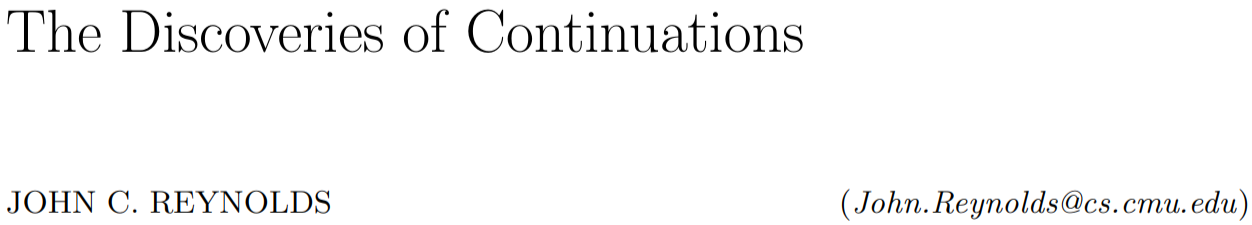
\includegraphics[width=0.6\textwidth]{figs/discoveries-of-continuations}
        \end{figure}
        \begin{itemize}
            \item Абстрактная концепция, зонтичный термин
            \item Придумано, чтобы дать денотационную (математическую) семантику \texttt{LABEL} и \texttt{GOTO}
        \end{itemize}
        \pause
        \begin{block}{Continuation (C. P. Wadsworth)}
            \centering
            \large
            \vspace{0.5em}
            ``The meaning of the rest of the program''
            \vspace{0.5em}
        \end{block}
        \begin{itemize}
            \item Если конкретнее, продолжение --- структура данных
            \item Содержит всё необходимое для вычислителя, чтобы продолжать вычисление
        \end{itemize}
    \end{frame}

    \begin{frame}[fragile]{Продолжения в языке выражений}
        \vspace{-1em}
        % Получили вычисление по действиям из начальной школы
        \begin{columns}[onlytextwidth]
            \begin{column}{0.465\textwidth}
                \begin{itemize}
                    \item Вычислитель ищет вычислимое подвыражение (redex)
                    \item Внешнее выражение сохраняется как ``выражение с дыркой'' --- продолжение
                    \item Продолжение возобновляется с результатом
                \end{itemize}
            \end{column}%
            \begin{column}{0.55\textwidth}
                \begin{figure}[h]
                    \centering
                    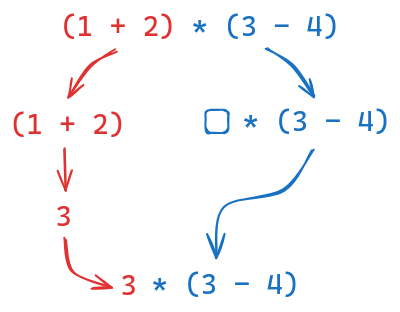
\includegraphics[width=0.7\textwidth]{figs/cont-expr}
                \end{figure}
            \end{column}
        \end{columns}
    \end{frame}

    \begin{frame}[fragile]{Операции, работающие с продолжениями}
        \vspace{1em}
        \begin{description}
            \item[\texttt{exit}] Выбрасывает продолжение программы
            \item[\texttt{break}] Возобновляет продолжение после цикла
            \item[\texttt{continue}] Возобновляет продолжение до цикла
            \item[\texttt{return}] Возобновляет продолжение вызывающей функции
        \end{description}
        \begin{figure}[h]
            \centering
            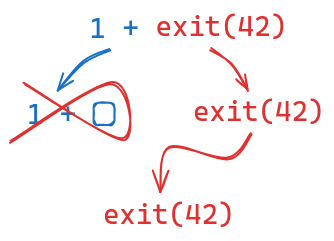
\includegraphics[width=0.35\textwidth]{figs/cont-exit}
        \end{figure}
    \end{frame}

    \begin{frame}[fragile]{Ограниченные продолжения (delimited continuations)}
        \begin{itemize}
            \item Продолжение целиком --- это не очень полезная и безопасная конструкция
            \item Как правило, работают с ограниченными продолжениями --- до некоторой точки
        \end{itemize}
        \begin{figure}[h]
            \centering
            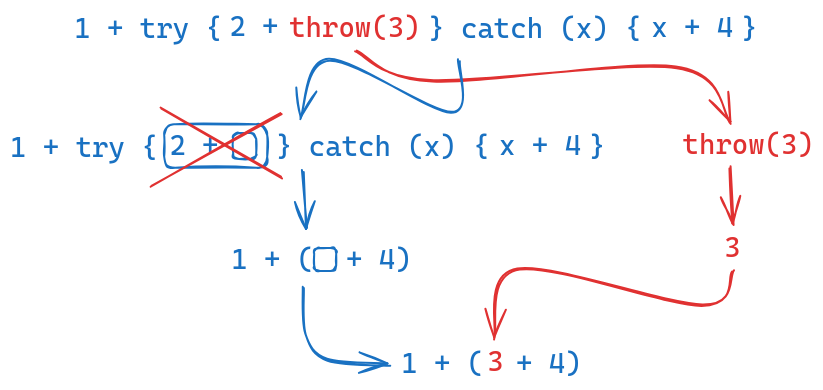
\includegraphics[width=0.8\textwidth]{figs/cont-try-catch}
        \end{figure}
    \end{frame}

    \begin{frame}[fragile]{Продолжения первого класса}
        % Хоть и звучит магически, это же кишки интерпретатора
        \begin{itemize}
            \item Для многих приложений нужно из программы иметь доступ к её продолжению
            \item Продолжение --- ``выражение с дыркой''\ldots
            \item Можно представить как функцию первого класса!
            \item Либо язык должен предоставлять специальные примитивы
            \item[\eg] \texttt{call-cc}, \texttt{shift/reset}, \texttt{prompt/control}
            \item Либо можно переписать программу в CPS
        \end{itemize}
    \end{frame}

    \begin{frame}[fragile]{Continuation passing style (CPS)}
        % Метафора криворукого друга
        \begin{itemize}
            \item В каждую функцию явно передаём продолжение --- что делать с результатом
            \item Будем в качестве аргумента принимать дополнительно функцию
            \item Вместо возвращения результата, будем передавать его в данную функцию
            \item Изоморфизм \mintinline{haskell}|a -> b #$\simeq$# (b -> r) -> (a -> r)| (следствие леммы Йонеды)
            \item \pause Обычный факториал
            \begin{minted}{haskell}
                fac :: Int -> Int
                fac n = if n <= 1 then 1 else n * fac (n - 1)
            \end{minted}
            \item \pause CPS-трансформированный факториал
            \begin{minted}{haskell}
                facCps :: Int -> (Int -> Int) -> Int
                facCps n #\framebox{k}# = if n <= 1 then k 1 else
                  facCps (n - 1) (\res -> k (res * n))
            \end{minted}
            \item \pause Пример вычисления
            \begin{minted}{haskell}
                facCps 3 k #$\rightsquigarrow$# facCps 2 (\res -> k (3 * res))
                #$\rightsquigarrow$# facCps 1 (\res -> k (3 * (2 * res))) #$\rightsquigarrow$# k (3 * (2 * 1))
            \end{minted}
        \end{itemize}
    \end{frame}

    \begin{frame}[fragile]{Асинхронное программирование, callback'и}
        \begin{itemize}
            \item Бывают долгие операции, например, запрос по сети
            \item Хотим, чтобы код делал что-то полезное, а не просто ждал
            \begin{minted}{scala}
                result <- queryInternet "hello"
            \end{minted}
            \item Вместо этого передадим callback и не будем ждать
            \begin{minted}{scala}
                queryInternet "hello" (\result -> processResult result)
            \end{minted}
            \item Ситуация быстро выходит из-под контроля --- callback hell
        \end{itemize}
        \begin{figure}[h]
            \centering
            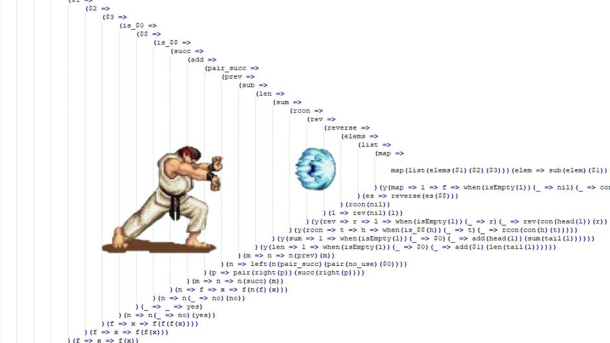
\includegraphics[width=0.4\textwidth]{figs/callback-hell}
        \end{figure}
    \end{frame}

    \begin{frame}[fragile]{Монада Cont, Futures}
        \begin{itemize}
            \item Монада --- это структура данных \mintinline{haskell}|F| с операцией
            \begin{minted}{haskell}
                andThen :: F a -> (a -> F b) -> F b
            \end{minted}
            \item Для структуры \mintinline{haskell}|Future a = (a -> r) -> r| можно определить \mintinline{haskell}|andThen| (монада \mintinline{haskell}|Cont|)
            \begin{minted}{haskell}
                andThen comp k = \k' -> comp \x -> (k x) k'
            \end{minted}
            \item Будем не принимать

        \end{itemize}
        % todo
    \end{frame}

    \begin{frame}[fragile]{Дефункционализация}
        \begin{itemize}
            \item Метод избавления от функций первого класса
            \item Для каждой функции первого класса заводим по конструктору данных
            \item Каждое применение заменяем на вызов интерпретатора
        \end{itemize}
        \begin{columns}[onlytextwidth]
            \begin{column}{0.485\textwidth}
                \begin{figure}[h]
                    \centering
                    \begin{tabular}{ll}
                        \mintinline{haskell}|(\x -> isRed x)| & \mintinline{haskell}|IsRed| \\
                        \mintinline{haskell}|(\x -> x == 42)| & \mintinline{haskell}|Equals 42| \\
                        \mintinline{haskell}|f value| & \mintinline{haskell}|apply fsym value|
                    \end{tabular}
                \end{figure}
            \end{column}\hfill%
            \begin{column}{0.485\textwidth}
                \begin{minted}{haskell}
                    data FSym = IsRed | Equals Int

                    apply sym x = case sym of
                      IsRed -> isRed x
                      Equals y -> x == y
                \end{minted}
            \end{column}
        \end{columns}
    \end{frame}

    \begin{frame}[fragile]{Дефункционализация продолжений}
        \begin{itemize}
            \item Дефункционализируем факториал
        \end{itemize}
        \vspace{-3em}
        \begin{columns}[onlytextwidth]
            \begin{column}[t]{0.485\textwidth}
                \begin{minted}{haskell}
                    #\color{white}lol#

                    fac :: Int -> Int
                    fac n = facCps n #\framebox{id}#

                    facCps :: Int -> (Int -> Int) -> Int
                    facCps n k = if n <= 1 then k 1 else
                      facCps (n - 1) #\framebox{(\textbackslash{}res -> k (res * n))}#
                \end{minted}
            \end{column}\hfill%
            \begin{column}[t]{0.485\textwidth}
                \begin{minted}{haskell}
                    data Cont = Halt | Cont Int Cont

                    fac :: Int -> Int
                    fac n = facCps n #\framebox{Halt}#

                    facCps :: Int -> Cont -> Int
                    facCps n k = if n <= 1 then prod k else
                      facCps (n - 1) #\framebox{(Cont n k)}#
                \end{minted}
            \end{column}
        \end{columns}
        \vspace{1em}
        \begin{itemize}
            \item \pause Дефункционализованное продолжение представляет собой просто список чисел (стек)
            \item Программный стек --- дефункционализированное продолжение
            \item \pause Умножение --- ассоциативно, можем поменять порядок операций
            \item Рефункционализируем и получим хвостовую рекурсию с аккумулятором --- цикл!
        \end{itemize}
        \vspace{0.5em}
        \begin{minted}{haskell}
            fac n = facAcc n 1
            facAcc n k = facAcc (n - 1) (n * k)
        \end{minted}
    \end{frame}

    \begin{frame}[fragile]{Корутины}
        \begin{itemize}
            \item Языковая реализация логических потоков исполнения
            \item Код, который может приостанавливаться и возобновляться в нужный момент
            \item Да, это всё про манипуляцию продолжениями
            \begin{minted}{kotlin}
                suspend fun <T> suspendCoroutine(block: (Continuation<T>) -> Unit): T
            \end{minted}
            \item Бесстековые (stackless) корутины
            \begin{itemize}
                \item C помощью CPS трансляции отбираем контроль у рантайма
                \item Экономим аллокации, сплющивая фреймы продолжений в машину состояний
                \item C++, Rust, C\#, Kotlin, JavaScript, Haskell\ldots
            \end{itemize}
            \item Стековые (stackful) корутины
            \begin{itemize}
                \item Стек --- продолжение
                \item Учим рантайм копировать стеки по требованию
                \item Haskell, Java, Go\ldots
            \end{itemize}
        \end{itemize}
    \end{frame}

    % todo зипперы и алгебраическая запись типа

    % todo реакт

    % todo алгебраические эффекты и хендлеры

    % todo заключение

\end{document}
